%% eval.tex
%% $Id: eval.tex 61 2012-05-03 13:58:03Z bless $

\chapter{Evaluation}
\label{ch:Evaluation}
%% ==============================
\section{Empirical analysis of the decomposition}

We are free to choose what states are substituted and used in the decomposition algorithm and further on, either the ones or the zeros from the label. Intuitively, there are less ones than zeroes in the original data, therefore less periods need to be found and less values to be mapped, which in turn should increase speed and effectiveness, therefore initially ones were substituted. For the empirical analysis of the decomposition, each edge of each graph of the collection is decomposed into periods and then the periods are collected until they align to give the original data. All the periods are evaluated and also visualized directly in code with the help of Lets-Plot\footnote{\url{https://lets-plot.org/}}.

\begin{figure}[h]
	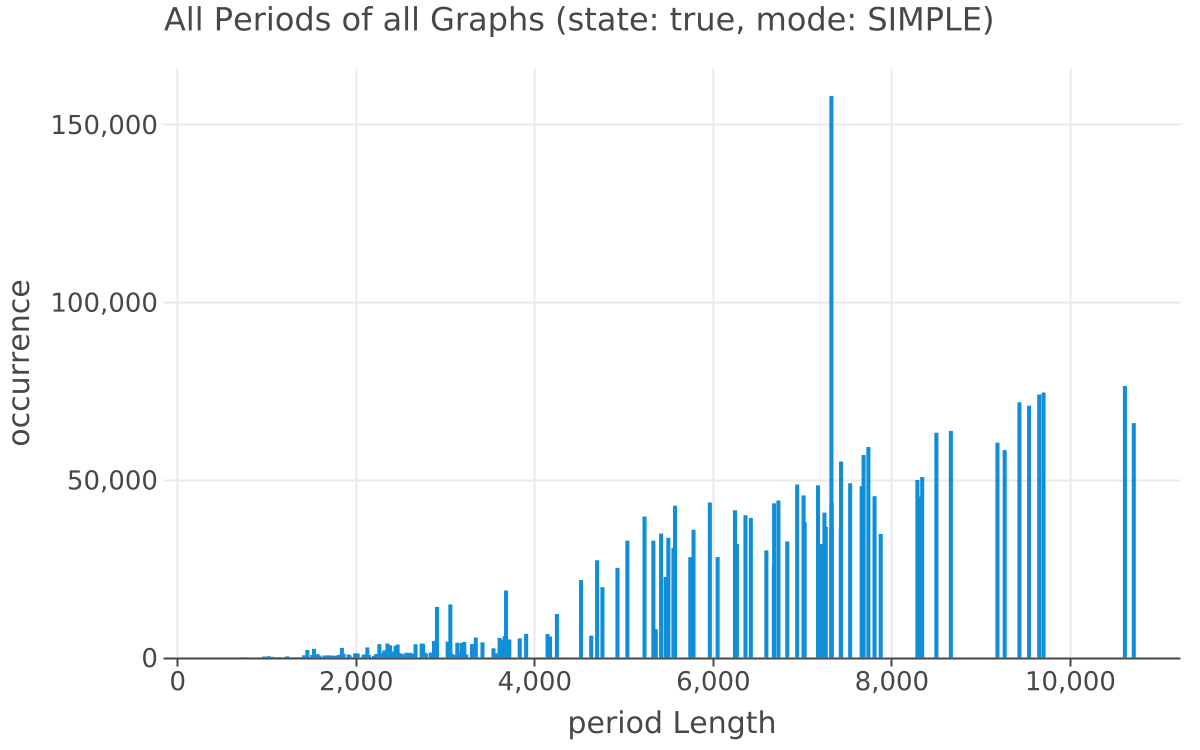
\includegraphics[width=\linewidth]{charts/all-graphs-bar-char-strue-mSIMPLE.png}
	\caption{A subfigure}
	\label{fig:plot-all-periods-true-state}
\end{figure}

In total, 3,126,993 values have been covered with a total of 2,854,922 periods, so on average a single period only covered 1.095 values from the input label. This is also visible in the bar chart in figure \ref{fig:plot-all-periods-true-state}, where there are some smaller periods present with a period length around 2000 but the main bulk has a period length larger than 4000. Switching the state to substitute to false, increases the amount of states to represent but also the chances of finding shorter periods which cover more than one value on average.

\begin{figure}[h]
	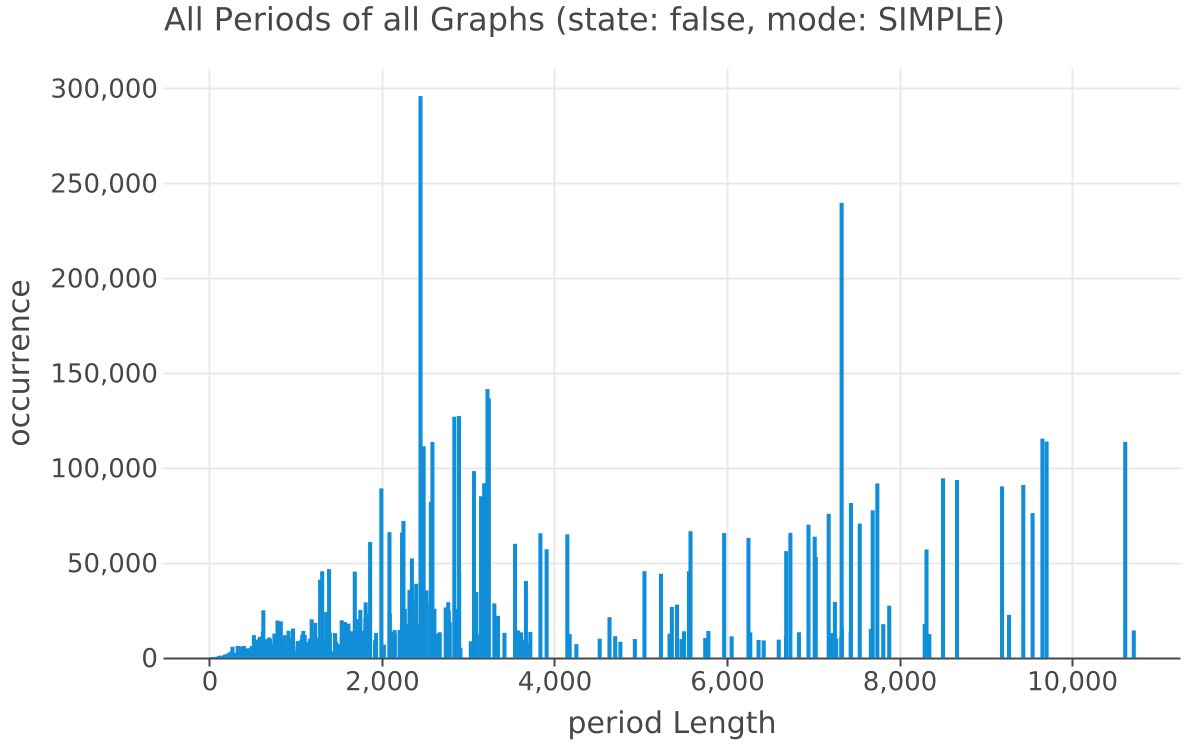
\includegraphics[width=\linewidth]{charts/all-graphs-bar-char-sfalse-mSIMPLE.png}
	\caption{A subfigure}
	\label{fig:plot-all-periods-false-state}
\end{figure}

Looking at the evaluation of substituting zeroes in figure \ref{fig:plot-all-periods-false-state}, a mixed image is visible. The amount of values to cover as well as the amount of periods increased to 20,077,026 values and a total of 7,341,229 periods. This means an improvement to 2.73 values per period on average but also a 7x increased amount of periods.

\begin{figure}[h]
	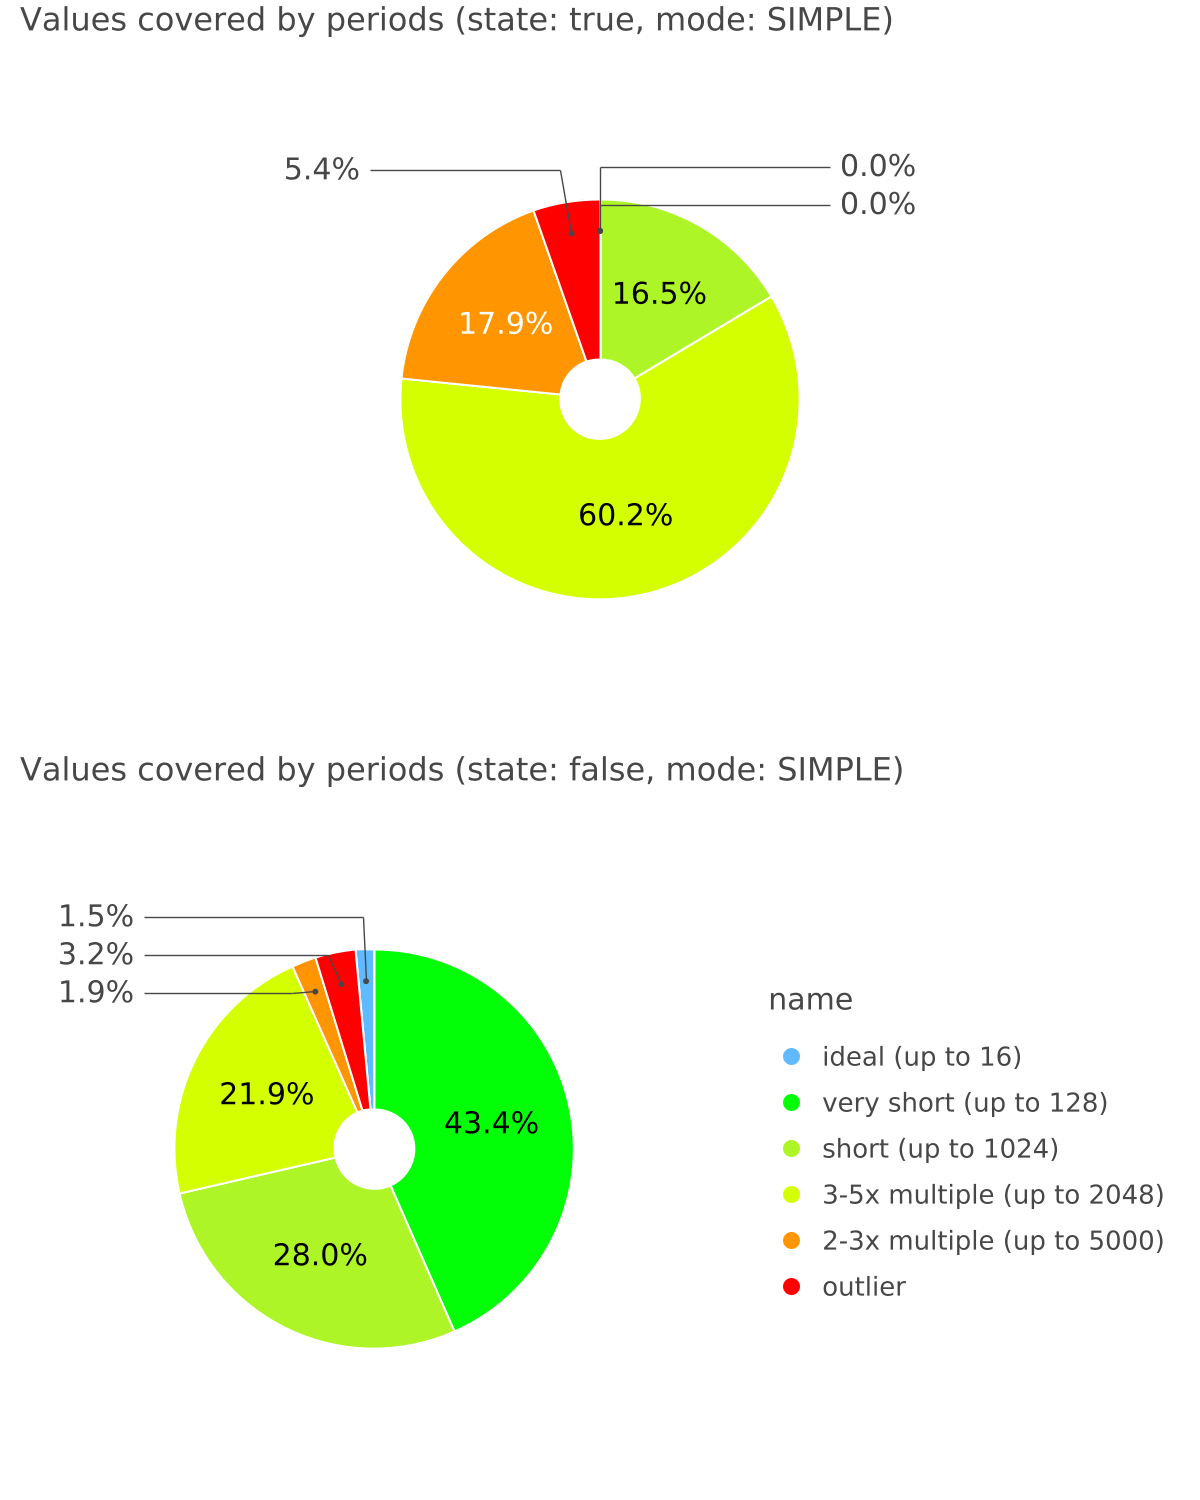
\includegraphics[width=\linewidth]{charts/all-covered-values-pie-chart-combined-ontop.png}
	\caption{A subfigure}
	\label{fig:sub2}
\end{figure}

%%% Local Variables: 
%%% mode: latex
%%% TeX-master: "thesis"
%%% End: 
